\documentclass{article}
\usepackage[UTF8]{ctex} % Required for inserting images
\usepackage{graphicx}
\usepackage{amsmath}

\begin{document}

\section{题目4.2}

    \begin{figure}[!h]
        \centering
        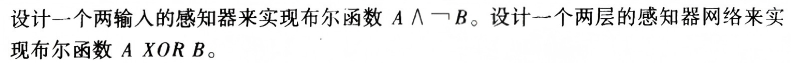
\includegraphics[width=1.2\linewidth]{image/4.2.png}
        \label{4.2}
    \end{figure}

    约定布尔值 True 用 1 表示,False 用 0 表示。感知器的激活函数为阶跃函数,即当加权和大于等于阈值 $\theta$(或 $w_0 + \sum w_ix_i \ge 0$)时,输出为 1,否则输出为 0。

    \paragraph{第 1 部分: 实现 $A \land \neg B$}~{}
    
    这是一个单层感知器可以解决的问题,因为该函数是线性可分的。\\

    \textbf{列出真值表}
    
    输入为 $x_1$ (代表 A) 和 $x_2$ (代表 B)。    
    \begin{center}
    \begin{tabular}{|c|c|c|c|}
    \hline
    \textbf{A ($x_1$)} & \textbf{B ($x_2$)} & \textbf{$\neg B$} & \textbf{$A \land \neg B$ (期望输出)} \\
    \hline
    0 & 0 & 1 & 0 \\
    0 & 1 & 0 & 0 \\
    1 & 0 & 1 & 1 \\
    1 & 1 & 0 & 0 \\
    \hline
    \end{tabular}
    \end{center}

    \textbf{建立不等式} 
    
    需要找到权重 $w_1, w_2$ 和阈值 $\theta$,使得: $w_1x_1 + w_2x_2 \ge \theta$ 时,输出为 1;否则输出为 0。
    
    根据真值表,得到以下不等式组:
    
    $w_1(0) + w_2(0) < \theta \implies 0 < \theta$
    
    $w_1(0) + w_2(1) < \theta \implies w_2 < \theta$
    
    $w_1(1) + w_2(0) \ge \theta \implies w_1 \ge \theta$
    
    $w_1(1) + w_2(1) < \theta \implies w_1 + w_2 < \theta$\\

    \textbf{求解权重和阈值}
    
    从 $w_1 \ge \theta$ 和 $w_1 + w_2 < \theta$ 可以推断出 $w_2$ 必须为负数。
    
    设定一个合适的阈值,例如 $\theta = 1$。那么不等式变为:$w_1 \ge 1$, $w_2 < 1$, $w_1 + w_2 < 1$。
    
    取 $w_1=1$。为了满足 $1 + w_2 < 1$,需要 $w_2 < 0$。
    
    取 $w_2=-1$。也满足 $w_2 < 1$。
    
    所以,一组可行的解是:$w_1 = 1, w_2 = -1, \theta = 1$。\\

    \textbf{设计方案}
    
    一个两输入的感知器,输入分别为 $x_A$ 和 $x_B$:
    
    \textbf{权重:} $w_A = 1, w_B = -1$
    
    \textbf{阈值:} $\theta = 1$
    
    \textbf{计算规则:} 当 $1 \cdot x_A - 1 \cdot x_B \ge 1$ 时输出 1,否则输出 0。

    \paragraph{第 2 部分: 实现 $A \text{ XOR } B$}~{}
    
    异或(XOR)函数不是线性可分的,无法用单个感知器实现,必须使用多层网络。一个常见的实现方法是利用逻辑等价式:
    \[ A \text{ XOR } B = (A \land \neg B) \lor (\neg A \land B) \]
    
    \textbf{网络结构设计} 
    
    构建一个两层的网络:

    \textbf{输入层:} 两个节点,代表 A 和 B。
    
    \textbf{隐藏层:} 两个感知器(神经元)。
        
        H1: 实现 $A \land \neg B$;
        H2: 实现 $\neg A \land B$
    
    \textbf{输出层:} 一个感知器(神经元)。
    
        O1: 将 H1 和 H2 的输出作为输入,实现 "或" (OR) 逻辑。\\
        
    \textbf{设计隐藏层感知器}
    
    \textbf{H1 ($A \land \neg B$):} 根据第一部分的解答设置:
        
        权重: $w_{A1} = 1, w_{B1} = -1$
        
        阈值: $\theta_{H1} = 1$
        
    \textbf{H2 ($\neg A \land B$):} 这个函数与上一个对称。一组解是:
        
        权重: $w_{A2} = -1, w_{B2} = 1$
        
        阈值: $\theta_{H2} = 1$\\
        
    \textbf{设计输出层感知器}
    
    O1 (OR):输出层感知器 O1 的输入是 H1 和 H2 的输出 $y_1$ 和 $y_2$。它需要实现 $y_1 \lor y_2$。
        
    真值表:(0,0) 输出 0,其他情况 (0,1), (1,0), (1,1) 均输出 1。\\

    不等式组:
    
    $w'_1 y_1 + w'_2 y_2 \ge \theta_{O1}$
        
    $w'_1(0) + w'_2(0) < \theta_{O1} \implies 0 < \theta_{O1}$
    
    $w'_1(0) + w'_2(1) \ge \theta_{O1} \implies w'_2 \ge \theta_{O1}$
    
    $w'_1(1) + w'_2(0) \ge \theta_{O1} \implies w'_1 \ge \theta_{O1}$

    设置 $\theta_{O1} = 1$。需要 $w'_1 \ge 1$ 且 $w'_2 \ge 1$。\\
   
    选择最简单的解:$w'_1 = 1, w'_2 = 1$。
        
        权重: $w_{H1\_O1} = 1, w_{H2\_O1} = 1$
        
        阈值: $\theta_{O1} = 1$

    \paragraph{最终设计方案:}~{}
    
    一个包含输入层、隐藏层和输出层的两层感知器网络。
    
    \textbf{输入层:} $x_A, x_B$
    
    \textbf{隐藏层:}
        
        神经元 H1:输入为 $(x_A, x_B)$,权重为 $(1, -1)$,阈值为 $\theta_{H1}=1$。

        神经元 H2:输入为 $(x_A, x_B)$,权重为 $(-1, 1)$,阈值为 $\theta_{H2}=1$。
        
    \textbf{输出层:}
        
        神经元 O1:输入为 H1 和 H2 的输出 $(y_{H1}, y_{H2})$,权重为 $(1, 1)$,阈值为 $\theta_{O1}=1$。\\
    
    这个网络结构可以成功实现 A XOR B 的功能。

\section{题目4.3}

    \begin{figure}[!h]
       \centering
       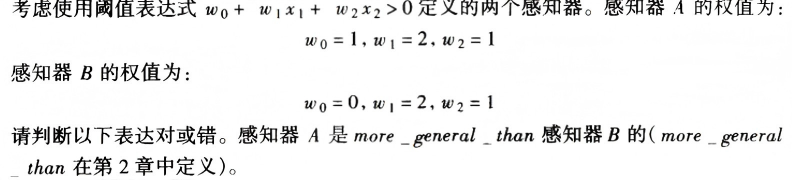
\includegraphics[width=1.2\linewidth]{image/4.3.png}
       \label{4.3}
   \end{figure}

    \paragraph{“more-general-than”的定义}~{}

    在概念学习中,一个假设(在这里是一个感知器)$h_A$ 比另一个假设 $h_B$ 更“泛化”(general),当且仅当所有被 $h_B$ 划分为正例的样本,也都被 $h_A$ 划分为正例。如果 $h_B$ 的正例集合是 $h_A$ 正例集合的子集,那么 $h_A$ 就比 $h_B$ 更泛化。

    \paragraph{分析两个感知器的分类规则}~{}
    感知器 A 将一个输入 $(x_1, x_2)$ 分类为正例,当且仅当满足:
            \[ 1 + 2x_1 + x_2 \ge 0 \]
    
    感知器 B 将一个输入 $(x_1, x_2)$ 分类为正例,当且仅当满足:
            \[ 2x_1 + x_2 \ge 0 \]


    \paragraph{逻辑推导}~{}
    
    判断“感知器 A is more-general-than 感知器 B”是否正确。根据定义,需要验证:是否所有被 B 划分为正例的样本,也都被 A 划分为正例?
    
    假设有一个任意的样本点 $(x_1, x_2)$ 被感知器 B 划分为正例。根据感知器 B 的规则,不等式 $2x_1 + x_2 \ge 0$ 成立。
    
    现在考察感知器 A 对这个样本点的分类。需要判断 $1 + 2x_1 + x_2$ 的值。
    
    因为 $2x_1 + x_2 \ge 0$,那么不等式的两边同时加 1,可得:
        \[ 1 + (2x_1 + x_2) \ge 1 + 0 \]
        \[ 1 + 2x_1 + x_2 \ge 1 \]
    
    由于 $1 > 0$,必然也满足 $1 + 2x_1 + x_2 \ge 0$。
    
    证明任何一个被感知器 B 划分为正例的样本,也一定会被感知器 A 划分为正例。
    
    \paragraph{寻找反例}~{}
    
    感知器 A 和 B 是否等价,如果不等价,A 就是严格地比 B 更泛化。我们需要找一个被 A 划分为正例,但被 B 划分为反例的样本。
    
    需要满足: $1 + 2x_1 + x_2 \ge 0$ 并且 $2x_1 + x_2 < 0$。
    
    令 $2x_1 + x_2 = -0.5$满足第二个条件。
    
    将它代入第一个条件:$1 + (-0.5) = 0.5 \ge 0$。也满足。\\
    
    例如,取点 $(x_1 = 0, x_2 = -0.5)$。
        
    对于感知器 A:$1 + 2(0) + (-0.5) = 0.5 \ge 0$。样本被划分为正例。
    
    对于感知器 B:$2(0) + (-0.5) = -0.5 < 0$。样本被划分为反例。
    
    说明存在被 A 划分为正例但被 B 划分为反例的样本。因此,A 的正例集合比 B 的正例集合更大,A 严格地比 B 更泛化。

    \paragraph{结论:} 该表述正确。

\end{document}
